%-------------------------------------------------------------------------------
% File: database.tex
%
% Author: Marco Pinna
%         Created on 06/08/2022
%-------------------------------------------------------------------------------
\chapter{Database}\label{ch:database}
A total of three databases have/has been created for the application:
\begin{itemize}
	\item the \texttt{votes} database, which is located in the central node and stores all the votes in encrypted for the whole duration of the election;
	\item the \texttt{polling stations} database, which is also located in the central node and stores the information related to each polling station, included their public keys;
	\item the \texttt{voter} database. Each polling station has its own voter database, containing the information related to each voter who is registered to said polling station. It contains the voters' personal details, necessary for the identification, as well as each voter's public key.
\end{itemize}

\section{Votes database}\label{sec:votes_db}
The \texttt{votes} database is a SQLite database located on the central node. It receives and stores in encrypted form all the votes cast by the voters during the election.\\
The database only consists of one table, \texttt{votes}, whose schema is the following:\\
\begin{figure}[H]
    \begin{center}
        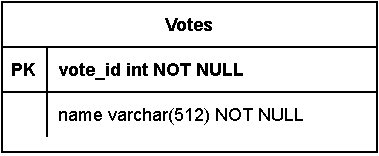
\includegraphics[scale=1]{img/votes_schema.pdf}
    \end{center}
    \vspace*{-0.5cm}
    \caption{Schema of the \texttt{votes} table.}
    \label{fig:votes_schema}
\end{figure}
The interaction with this database is handled by the \texttt{DatabaseManager} Java class which offers an interface to perform CRUD operations.\\
The module that interact with the \texttt{votes} database are the \texttt{CentralStationDaemon} to add the votes to the database and the \texttt{CentralStationDashboard} to obtain the election turnout. %TODO check if something is missing
An example of how the table might appear during the election is the following:

TODO: add example of database

\section{Polling stations database}\label{sec:polling_stations_db}
The \texttt{polling stations} database is a Mnesia database located on the central node. It stores the information related to each polling station.\\
The database only consists of one table, \texttt{pollingStation}, whose schema is the following:\\
\
\begin{figure}[H]
    \begin{center}
        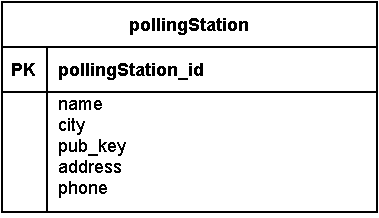
\includegraphics[scale=1]{img/pollingstation_schema.pdf}
    \end{center}
    \vspace*{-0.5cm}
    \caption{Schema of the \texttt{pollingStation} table.}
    \label{fig:pollingstation_schema}
\end{figure}

It is worth noting that ``Mnesia tables \textit{have no built-in type constraints}, as long as you respect the tuple structure of the table iteslf."\footnote{\textit{Learn you some Erlang for great good},Fred Hébert, 2013, p. 514.}.\\
The schema of this table is specified in the Erlang header file \texttt{pollingStation.hrl} while \texttt{pollingStation.erl} offers functions to interact with it, e.g. to add a polling station to the database or to retrieve a polling station public key given its id.\\
An example of how the table might appear during the election is the following:

TODO: add example of database

\section{Voter database}\label{sec:voters_db}
A \texttt{voter} Mnesia database is located on each one of the polling station nodes. Each of them stores the information related to every voter who is registered to that polling station.\\
The database only consists of one table, \texttt{voter}, whose schema is the following:\\
\
\begin{figure}[H]
    \begin{center}
        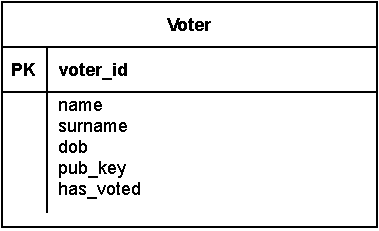
\includegraphics[scale=1]{img/voter_schema.pdf}
    \end{center}
    \vspace*{-0.5cm}
    \caption{Schema of the \texttt{voter} table.}
    \label{fig:voter_schema}
\end{figure}

The schema of this table is specified in the Erlang header file \texttt{voter.hrl} while \texttt{voter.erl} offers functions to interact with it, e.g. to add a voter to the database, to retrieve a voter's public key given their id or to set the flag \texttt{has\_voted} to \textit{true} once the voter has cast their vote.\\
An example of how the table might appear during the election is the following:

TODO: add example of database
